\documentclass[a4paper,10pt]{article}

\usepackage[utf8]{inputenc}
\usepackage{t1enc}
\usepackage[spanish]{babel}
\usepackage[pdftex,usenames,dvipsnames]{color}
\usepackage[pdftex]{graphicx}
\usepackage{amsmath}
\usepackage{amsfonts}
\usepackage{amssymb}
\usepackage{listings}
\lstset{language=C}
\lstset{showstringspaces=false}
\lstset{basicstyle=\ttfamily,}

\usepackage{float}
\floatstyle{boxed} 
\restylefloat{figure}

\begin{document}


\renewcommand{\lstlistingname}{C\'odigo Fuente}
\lstloadlanguages{Octave} 
\lstdefinelanguage{MyPseudoCode}[]{Octave}{
	deletekeywords={beta,det},
	morekeywords={repmat}
} 
\lstset{
	language=MyPseudoCode,
	stringstyle=\ttfamily,
	showstringspaces = false,
	basicstyle=\footnotesize\ttfamily,
	commentstyle=\color{gray},
	keywordstyle=\bfseries,
	numbers=left,
	numberstyle=\ttfamily\footnotesize,
	stepnumber=1,                   
	framexleftmargin=0.20cm,
	numbersep=0.37cm,              
	backgroundcolor=\color{white},
	showspaces=false,
	showtabs=false,
	frame=l,
	tabsize=4,
	captionpos=b,               
	breaklines=true,             
	breakatwhitespace=false,      
	mathescape=true
}
\begin{titlepage}
        \thispagestyle{empty}
        \begin{center}
                
\includegraphics{./images/itba.jpg}
                \vfill
                \Huge{Sistemas Operativos}\\
                \vspace{1cm}
                \huge{Trabajo Práctico Especial Nº1}\\
        \end{center}
        \vspace{2cm}
        \large{
                \begin{tabular}{lcrc}
                        \textbf{Alvaro Crespo} & & 50758 & \ \ \texttt{acrespo@alu.itba.edu.ar}\\
                        \textbf{Juan Pablo Civile} & & 50453 & \ \ \texttt{jcivile@alu.itba.edu.ar}\\
                        \textbf{Darío Susnisky} & & 50592 & \ \ \texttt{dsusnisk@alu.itba.edu.ar}\\
                        \\ 
                \end{tabular}
        }
        \vfill
        \flushright{12 de Septiembre del 2011}
\end{titlepage}

\setcounter{page}{1}

\tableofcontents
\newpage
\section{Introducción}
El objetivo de este trabajo es familiarizarse con el uso de sistemas cliente-servidor concurrentes, implementando el servidor mediante la creación de procesos hijos 
utilizando \textit{fork()} y mediante la creación de \textit{threads}. Al mismo tiempo, ejercitar el uso de los distintos tipos de primitivas de sincronización y 
comunicación de procesos (IPC) y manejar con autoridad el \textit{filesystem} de Linux desde el lado usuario.

\newpage
\section{Esquema de la aplicación}

A la hora de encarar el problema en cuestión, una de las primeras cosas a plantearse era el diseño de la aplicación. Dada la naturaleza y los objetivos planteados para este
 trabajo práctico, era necesario poder identificar que partes de nuestra simulación iban a ser procesos paralelos y cuales tenía coherencia implementarlas como \textit{threads}.
  En este debate, también fue importante no forzar la separación de procesos cuando el problema no lo requería (por ejemplo que cada avión fuera un proceso independiente no agregaba 
  nada y generaba mucha complejidad, por lo que se optó por implementarlos como \textit{threads}).\\ 

En un primer análisis, identificamos como potenciales procesos paralelos de nuestro programa al control del flujo principal del programa, a los parsers, al mapa, a las aerolíneas y
 a los aviones. Luego de cierto debate, vimos que la relación entre el flujo principal, los parsers y el mapa era demasiado fuerte, pues, la combinación de estas tres cosas iban a 
 controlar el flujo de la simulación en sí. Inclusive, estas partes tenian una secuencia bastante marcada. Así, se decidió que estos elementos que originalmente bien podrían haber 
 sido planteado como procesos paralelos, era más intuitivo y coherente escribirlo como uno solo.\\

Por otra parte, la aerolínea y los aviones nos resulto intuitivo implementarlo como un proceso aparte. La siguiente decisión tomada fue que los aviones debian ser \textit{threads}
 de los procesos aerolinea. Pues nos resultó necesario implementarlo de esta manera ya que la relación entre una aerolínea y sus aviones era constante, ya que un avión es parte
  de una aerolínea.\\

A continuación se presentan esquemas que representan las tomas de decisiones respecto al esquema de la simulación recién mencionadas:

\newpage
\section{Modelo OSI}

El modelo OSI es un modelo que estandariza la forma de diseñar un programa y como comunicar diferentes programas. Como se puede ver en el esquema\\
 (INCLUIR ESQUEMA)\\
 el modelo OSI cuenta con 7 capaz aunque dadas las funcionalidades de nuestra aplicación nuestro programa solo cuenta con las primeras cuatro implementadas (e inclusive, dos de las
  mismas están implementadas como una). Esto se debe a que nuestro programa no se comunica con otros programas, reduciendo así las capas del modelo OSI implementadas por nosotros.\\

El modelo OSI es muy útil ya que permite realizar las diferentes partes de una aplicación por separado sin mezclar información innecesaria y de esta manera las implementaciones 
en cada capa son independientes del resto. Por último, la separación en capaz mejora ampliamente la claridad del código.\\

En nuestro caso, la capa de aplicación es la encargada de realizar el flujo y la lógica de la aplicación en sí. Las capas de presentación y sesión estan implementadas como una sola,
 la capa de Marshalling. Esta se encarga de recibir los datos que se desean transmitir a otro proceso y dejarlos en estructuras de modo tal que la capa de Marshalling de otro proceso 
 lo pueda entender. Nuestra última capa implementada es la de transporte, que es la que se encarga de utilizar los diferentes tipos de \textit{IPCs} para comunicar procesos.\\

Notesé que es de suma importancia la separación en capas ya que, por ejemplo, gracias a esto fue posible implementar los distintos tipos de \textit{IPCs} sin importar el resto de las implementaciones.\\

\newpage
\section{Interfaz de comunicación(???)}
Presentar las distintas interfaces que tuvimos...
Creo que fueron tres en total... 
Criterios de elección Y de descarte...
CHAMPO esta es TU parte, te llama a gritosss jeje.

\newpage
\section{Problemas encontrados(???)}

Uno de los primeros problemas con los que nos topamos, fue el hecho de que los archivos de configuración de los cuales la aplicación debía levantar la información, tenían un formato
bastante díficil para trabajar con el lenguaje C. Al no contar con una estructura que pueda ir agregando elementos a una colección y cambiando de tamaño dinámicamente, debimos 
implementar nuestra propia estructura, \textit{Vector}. Esto probó ser muy útil más adelante ya que la utilizamos en otros sectores del programa.\\

Otro problema con el formato de los archivos de configuración, fue que los límites de las ``iteraciones'' se marcaban con líneas en blanco, y al parecer hay problemas al querer leer el 
$\backslash n$ con $fscanf$. Para lidiar con esta situación, recurrimos a la única solución que encontramos, aunque en términos de código no es muy elegante.\\

Otro problema encontrado, se relaciona con el testeo. Una vez implementadas las 4 implementaciones de la interfaz de IPC, diseñamos un pequeño test inicial, para detectar fallas en una 
etapa temprana. El test no era del todo básico, pero tampoco era muy agresivo. En ese momento, nos concentramos en que las implementaciones efectivamente funcionaran (comunicaran
 procesos). Al no haber hecho un test más exhaustivo, a la hora de testear la aplicación completa como un todo, surguieron algunos pequeños problemas relacionados con la 
 comunicación entre procesos que nuestro test inicial no había logrado detectar.\\

\newpage
\section{Conclusiones}

Queda claro que este trabajo podría haberse realizado sin necesidad de recurrir al procesamiento paralelo y a la comunicación entre procesos. Pero al haberlo 
hecho de de esta forma, la experiencia adquirida y el aprendizaje resulta mucho más significativo. Por varias razones:

\begin{itemize}
\item la experiencia adquirida al trabajar con varios procesos corriendo al mismo tiempo, al igual que varios \textit{threads}.
\item la comunicación entre estos procesos.
\item la separación en capas, consecuencia necesaria, que agrega mucha claridad al código y conceptualmente, al diferenciar claramente las responsabilidades.
\item la familiarización con los estándares \textit{POSIX} y \textit{System V}, o el simple de hecho de trabajar contra interfaces predefinidas y respetando
      un estándar predefinido.
\end{itemize}

Con respecto al uso de \textit{threads}  y procesos, nos topamos con una fuerte diferencia entre utilizar unos y otros. Por ejemplo, el uso de variables globales 
en un \textit{thread} debe ser llevado a cabo con mucho cuidado, ya que el estado global, o \textit{Data Segment}, es compartido por los demás \textit{threads} del mismo
proceso. Esto no es así con los procesos, cuyo estado global es propio y solo visible a ellos mismos. Por suerte, el \textit{stack} no es compartido por distintos \texit{threads}
los que les da un cierto grado de independencia, para que realicen distinas tareas. Otra diferencia que notamos, tiene que ver con la sincronizacíon. Mientras que un
simple \textit{lock} de un \textit{mutex} en la mayoría de los casos era lo único que se debía hacer para sincronizar \textit{threads}, para procesos se requirió el uso
de técnicas más avanzadas como semáforos.

Una vez terminado el trabajo, surgió la pregunta de cual era la implementación de IPC más rápida. Como nos dimos cuenta más tarde, esto no es tan fácil de determinar. 
Esto se debe a que el rendimiento de cada implementación varía dependiendo de la ejecución debido al procesamiento paralelo y el cual no es determínistico. Es decir, no 
es siempre se reproduce exactamente la misma ejecución dadas las mismas condiciones iniciales. \\
A pesar de lo dicho anteriormente, es posible, observar ciertas tendencias en los tiempos de ejecución. El siguiente gráfico muestra los distintos tiempos obtenidos por 
cada implementación para una serie de 4 simulaciones. La simulación 1 es la que presenta los menores tiempos, con 5 ciudades, 2 aerolíneas y 8 aviones en total.
La simulación 2, presenta una configuración similar aunque, en general, tarda más en terminar debido a una menor cantidad de aviones. Sus parámetros son
5 ciudades, 1 aerolínea y 3 aviones. La simulación 3, cuenta con 10 ciudades, 10 aerolíneas y 40 aviones en total, por lo que el tiempo de ejecucón, como es de 
esperar es un poco superior. Finalmente, la simulación 4 es la más intensiva, ya que tiene la configuración límite, con 50 ciudades, 10 aerolíneas, y un total de
100 aviones. Esta es, como se puede ver, la que presenta los mayores tiempos de ejecución.\\
Cabe aclarar, que debido a la variación que sufren de ejecución en ejecución nos pareció prudente tomar el promedio de 100 ejecuciones para cada simulación. 

\begin{figure}[H]
\begin{center}
 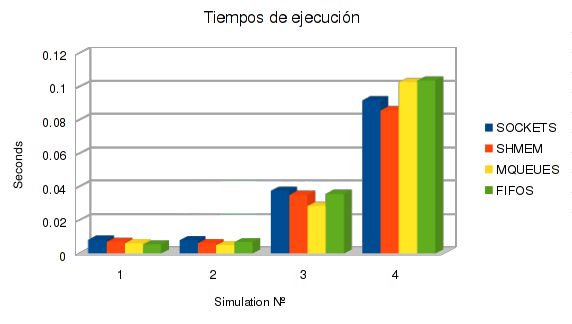
\includegraphics[scale=0.75]{./images/runningTimesChart.png}
 % runningTimesChart.png: 572x324 pixel, 96dpi, 15.13x8.57 cm, bb=0 0 429 243
  \caption{Comparación de los tiempos de ejecución de cada implementación.}
\end{center}
\end{figure}

En base a estos datos, pudimos concluir que en general la de \textit{shared memory} es la implementación con mejores tiempos, seguido de la de \textit{socket}. Aunque,
como puede observarse, para las primeras simulaciones, las menos intensivas, las implementaciones de \textit{message queues} y \textit{fifos} parecen tener mejores
tiempos. Después de analizar los datos, nuestra explicación es que, en esos casos el mayor \textit{overhead} que tienen las implementaciones como \textit{socket} y 
\textit{shared memory}, hacen que sus tiempos de ejecución sean levemente mayores. Pero, para simulaciones más intensivas, como por ejemplo la número 4, ese
 \textit{overhead} se torna despreciable, revelando los resultados que se observan en el gráfico: esas implementaciones terminan siendo más rápidas.\\


\newpage     
\section{Referencias}

\begin{itemize}
  \item Material provisto por la cátedra.
  \item UNIX system programming. Second Edition. Keith Havilland, Dina Gray, Ben Salama.
  \item http://cplusplus.com/cir
  \item http://beej.us/guide/bgipc/output/html/multipage/unixsock.html
  \item https://computing.llnl.gov/tutorials/pthreads/
  \item https://computing.llnl.gov/tutorials/parallel\_comp/
  \item http://www.csc.villanova.edu/~mdamian/threads/posixsem.html
  \item http://www.cs.cf.ac.uk/Dave/C/node25.html
  \item http://www.users.pjwstk.edu.pl/~jms/qnx/help/watcom/clibref/mq\_overview.html
  \item http://linux.die.net/man/7/mq\_overview
\end{itemize}
   
\end{document}
